\section{Introduction} % (fold)
\label{cha:introduction}

Object retrieval is a main topic in the research area of computer vision. Most methods for finding objects are designed specifically for certain subtopics, such as retrieving one type of objects only, categorizing the scene of the image, or discerning foreground objects from the background. For each of these subtopics, the object finding task is modeled in a certain way. Three very common models are image classification, image segmentation, and object detection.

In image classification (Figure~\ref{fig:classification}), the object finding task is represented as the task of predicting the class of a whole image. The prediction is some measure of how likely it is for an image to belong to a certain class. This task is useful when the image as a whole is of importance, for example when a user is looking for images of a certain topic.

Image segmentation is different from image classification, because for each pixel in the image, a class label has to be found.(Figure~\ref{fig:segmentation}) This task is more complex than classification, because there is less information available for a small patch of the image than for the image as a whole. Therefore, the context of each segment becomes more important for a good classification of objects. Image segmentation might be useful when trying to find the distinction between foreground and background, for example.

Object detection (Figure~\ref{fig:detection}) is similar to both image classification and segmentation, and lies somewhere in between these tasks. Detection is the task of pinpointing areas on an image where objects are, and of which class this object is. Detection is more specific than classification, because the objective is not only to give a class label, but also an indication of the object's location. This indication is not as specific however as in the segmentation task, because the goal is not to define a class for all pixels in the images, but only for the foreground objects. the indication of the object's location can be given in a number of ways, but the most common one is to give a rectangular bounding box that envelops the object \cite{pascal-voc-2007}. Object detection is useful when you are interested in only specific parts of the image, for example in tasks like face detection.

\begin{figure}[hbt]
    \centering
    \begin{subfigure}[b]{0.3\textwidth}
        \centering
        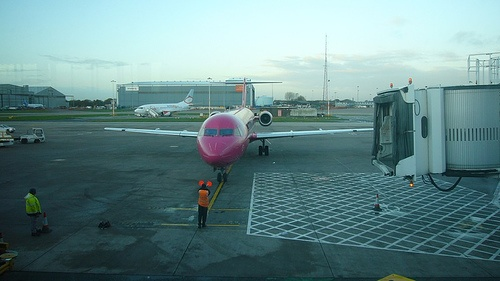
\includegraphics[width=\textwidth]{000032}
        \caption{Classification}
        \label{fig:classification}
    \end{subfigure}%
    ~ %add desired spacing between images, e. g. ~, \quad, \qquad etc.
      %(or a blank line to force the subfigure onto a new line)
    \begin{subfigure}[b]{0.3\textwidth}
            \centering
            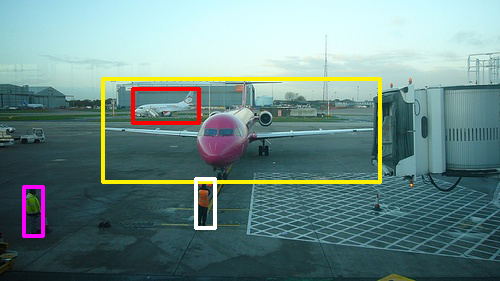
\includegraphics[width=\textwidth]{000032-det}
            \caption{Detection}
            \label{fig:detection}
    \end{subfigure}
    ~ %add desired spacing between images, e. g. ~, \quad, \qquad etc.
      %(or a blank line to force the subfigure onto a new line)
    \begin{subfigure}[b]{0.3\textwidth}
            \centering
            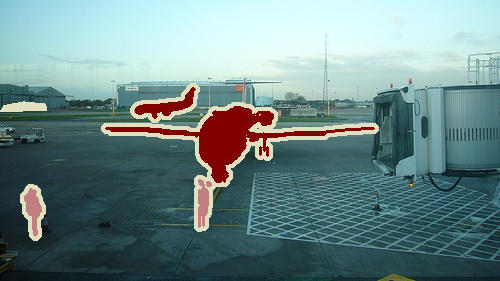
\includegraphics[width=\textwidth]{000032-clsseg}
            \caption{Class-segmentation}
            \label{fig:segmentation}
            \end{subfigure}
    \caption{Three Computer Vision tasks for the same image. If the question is to find persons and airplanes, in a classification task \textbf{(a)} it would be enough to classify the image as a whole as containing both classes. In a detection task \textbf{(b)} bounding boxes need to be given that neatly envelop the objects and have the correct class label. In a class-segmentation task \textbf{(c)}, every pixel should be labeled correctly ``airplane'', ``person'' or ``background'' (transparent in this case). Note that this segmentation image has a blank label for areas that are either on the boundary between different classes, or difficult to classify (at the left side of the image). \cite{pascal-voc-2007}}
    \label{fig:clsdetseg}
\end{figure}

These kinds of algorithms can be used in a broad range of applications. Image retrieval from the internet can be improved by using high level visual data next to textual data such as the filename or context of an image in a web page, especially as the amount of images on the internet grows much faster than they can be for example tagged by useful keywords. Various dedicated systems might use object recognition. For example, in robotics object detection might be used to determine where in the range of the robot certain objects are (and to interact with them accordingly). Another application field is object tracking in video footage. If objects can be successfully detected in single images, it is possible to use this information in an image sequence to learn the trajectories of objects within the sequence. This is useful in surveillance settings, or to gather individual statistics of players in team sports. \cite{benfold2011stable, ekin2003automatic, lipton1998moving}

While most humans have little difficulty categorizing visual input, recognizing objects or classes of objects, and tracking objects in continuous sequences through time, object recognition is regarded a difficult task. A computer basically ``sees'' an image as a bunch of numbers representing color values for each image pixel. When the image is not an exact copy of a known image, let alone an image of an object not seen before by the computer, it becomes hard to see sometimes crucial similarities. In an average recognition setting, this is the case almost all the time. When comparing images of a certain object of interest, the images tends not to be at the exact same location all the time, the lighting conditions vary, just like the viewpoint and distance of the camera, the camera quality, the image size. The object might be cut off by the edge of the image, or may be occluded by another object. When multiple objects of the same class need to be compared the issues become even bigger. The intra-class variety might be huge (think of all different kinds of chairs you have ever encountered), causing a large variance of appearance.

Therefore, higher level representations are needed to compare images, objects, and classes of objects. To this end, several kinds of image features have been developed that can describe parts of images at a higher level. These features usually cover a small part of the image, and describe numerically what this part looks like. For example, sharp color contrast, or the occurrence of lines, corners or blobs might be of interest, just like the size and direction of these properties. The features should usually be invariant to a number of (irrelevant) variables, and be covariant to important ones. These features make it easier to compare images and objects, because the question becomes: ``Which class' features do the features of this image resemble most?''

A number of different approaches have been developed to find a way to answer this question, or basically to classify images or objects. Usually these involve the analysis of a number of labeled images (the training phase), in which a model is learned for classifying new images. in the test phase, unlabeled query images are subjected to this model, and a decision is made which class is most likely.

For image classification, recently the Naive Bayes Nearest Neighbor (NBNN) \cite{boiman2008defense} approach has gained popularity. \cite{becker2012codebook, behmo2010towards, mccann2012local, timofte2012iterative, tuytelaars2011nbnn, wang2011improved, zhang2010random} Boiman \emph{et al.} apply the simple nature of nearest-neighbor classification to build a state-of-the-art image classification method. They show that a Nearest-Neighbor based approach for image classification has a number of appealing properties. In the first place, Nearest Neighbor is a so-called ``lazy'' classification method, meaning that it does not need a separate phase in which it learns a model. It does not build a model for a decision boundary based on the evidence given, but is just compares each query directly with this evidence. This also makes the method parameter-free, meaning that there are no parameters needed that influence the model that is made.

Because no model is learned, the raw evidence is of much importance in NBNN, therefore the more evidence is available, the better. Parametrized methods benefit from little but good evidence, but without a learning step, the quantization error this gives is very harmful. Furthermore, Boiman shows that query images should not be compared to evidence images, but to the aggregated evidence classes, image-to-class distance.

Among improvements by others, McCann \& Lowe \cite{mccann2012local} have come up with an adaptation of NBNN which looks at the local surroundings of image features in the NN-space across all classes in stead of a class-by-class approach. This Local NBNN (LNBNN) approach uses more than one single nearest neighbor to find object-to-class distances to multiple classes at once, making the process more efficient and the performance better. 

In this thesis I will explore the possibilities of extending the NBNN method from image classification to object detection. I combine McCann \& Lowe's LNBNN based object-to-class distance estimation with exemplar-model object detection \cite{becker2012codebook, chum2007exemplar}. To do this, each object descriptor taken during training is regarded as an exemplar. It refers to a certain part of the object it was sampled from. In this way, bounding box hypotheses can be made from descriptors in a test image and their nearest neighbor exemplars. These hypotheses can be clustered to form detections. In this regard, single-link agglomerative clustering as used by Becker \emph{et al.} \cite{becker2012codebook} is compared with quickshift mode finding clustering. \todo[fancyline]{need reference}

The experiments are performed on both a composed dataset of motorbike images (TUD Motorbikes) \cite{becker2012codebook, fritz2005integrating}, and on the more challenging VOC2007 object detection task \cite{pascal-voc-2007}.

The results show that exemplar-LNBNN detection is an improvement over earlier attempts to apply NBNN to an object detection task \cite{becker2012codebook}. Furthermore, the use of the quickshift algorithm a more theoretically sound clustering algorithm is shown to be justified. Nevertheless, the experiments also expose some vulnerabilities of the approach. The benefit of not having a learning phase, and therefore a short ``training'' time is compensated by a larger memory consumption (no efficient model to compress the evidence data) and a longer time to perform detection (comparison of each image feature to a large set of evidence features). Regardless of some efficiency improving measures, this remains a problem when it comes to large tests.

Section~\ref{cha:related_work} gives an overview of related work on the various parts of this task. In Section~\ref{cha:naive_bayes_nearest_neighbor} I will discuss the details of the NBNN method, and the assumptions under which it works. In Section~\ref{cha:object_detection} the theory behind exemplar-based modeling will be explained. The link between the two methods will be made in Section~\ref{cha:linking}. In Section~\ref{cha:experimental_setup} the experiments will be elaborated, after which the results are given. In Section~\ref{cha:analysis_of_results} these results are discussed and analyzed. Finally, in Section~\ref{cha:conclusion} conclusions will be drawn and discussed.

% section introduction (end)